\documentclass[a4paper,twocolumn]{article}
\usepackage[a4paper,left=30mm,right=30mm,top=30mm,bottom=32mm,columnsep=7.5mm]{geometry}
\usepackage{fontspec}
\setmainfont{TeX Gyre Termes}
\setsansfont{TeX Gyre Heros}
\usepackage{graphicx}
\usepackage{booktabs}
\usepackage{array}
\usepackage{xurl}
\urlstyle{same}
\usepackage[hidelinks]{hyperref}
\usepackage{microtype}
\usepackage{needspace}
\usepackage{fancyhdr}
\newfontfamily\cjkfont{HaranoAjiMincho-Regular.otf}
\renewcommand{\normalsize}{\fontsize{9pt}{11pt}\selectfont}
\setlength{\parindent}{1.5em}
\setlength{\parskip}{0pt}
\newcommand{\tablefont}{\fontsize{8pt}{10pt}\selectfont}
\renewcommand{\floatpagefraction}{0.7}
\renewcommand{\topfraction}{0.9}
\pagestyle{fancy}
\fancyhf{}
\renewcommand{\headrulewidth}{0pt}
\fancyfoot[C]{\fontsize{9pt}{11pt}\selectfont\thepage}
\fancypagestyle{plain}{\fancyhf{}\renewcommand{\headrulewidth}{0pt}\fancyfoot[C]{\fontsize{9pt}{11pt}\selectfont\thepage}}
\newcommand{\chap}[2]{\par\vspace{10pt}\needspace{4\baselineskip}\noindent{\sffamily\bfseries\fontsize{11pt}{13pt}\selectfont #1. #2\par}\vspace{4pt}\nopagebreak\noindent}
\newcommand{\chapx}[1]{\par\vspace{10pt}\needspace{4\baselineskip}\noindent{\sffamily\bfseries\fontsize{11pt}{13pt}\selectfont #1\par}\vspace{4pt}\nopagebreak\noindent}
\newcommand{\secn}[3]{\par\vspace{7pt}\needspace{3\baselineskip}\noindent{\sffamily\bfseries\fontsize{10pt}{12pt}\selectfont #1.#2 #3\par}\vspace{3pt}\nopagebreak\noindent}

\begin{document}
\twocolumn[{%
{\raggedleft\fontsize{8pt}{10pt}\selectfont SEDA GENERATIVE AI PAPERS, 2026\par}
\vspace{16pt}{\noindent\sffamily\bfseries\fontsize{10pt}{12pt}\selectfont Generative AI paper\par}
\vspace{8pt}{\noindent\sffamily\bfseries\fontsize{14pt}{18pt}\selectfont The Relationship Between Mathematics Anxiety and Mathematics Achievement in Primary and Lower Secondary Students: A Meta-Analysis\par}\vspace{6pt}
{\noindent\bfseries\fontsize{11pt}{14pt}\selectfont Society for Educational Data Analysis (SEDA)\par}\vspace{8pt}
{\noindent\itshape (The Japanese version of this paper, with identical content, is available at \url{https://raw.githubusercontent.com/k518-2026/MetaAnalysisToWP/main/reports/2026-10-06-math-anxiety-achievement/paper-ja.pdf}. Published October 6, 2026.)\par}\vspace{8pt}
{\noindent\fontsize{8pt}{10pt}\selectfont\textbf{\textit{Abstract}} Mathematics anxiety is a feeling of tension about mathematics, and understanding how it relates to achievement helps teachers in primary and lower secondary schools support their students. Using an automated workflow in which every extracted number was verified against the full text, 10 open-access studies (\textit{N} = 5389) were pooled with a random-effects model. The pooled effect was \textit{r} = \ensuremath{-}.34, 95\% CI [\ensuremath{-}.49, \ensuremath{-}.17], with \textit{I}² = 96.9\%. Higher mathematics anxiety was generally linked with lower achievement, but the size of the link varied widely, so teachers should treat it as a correlation rather than a proven cause.\par}\vspace{2pt}
{\noindent\fontsize{8pt}{10pt}\selectfont\textbf{\textit{Keywords}} meta-analysis, mathematics anxiety, mathematics achievement, primary education, lower secondary education, correlation\par}\vspace{10pt}
}]
\chap{1}{Introduction}
\noindent Mathematics is taught to all children in primary and lower secondary schools, yet many students feel tense or worried when they work on it. Such feelings are usually called mathematics anxiety. In school, mathematics anxiety is typically measured by asking students to rate how uneasy they feel in situations that involve numbers, lessons and tests. Because teachers meet students of many ages and backgrounds, they need to know whether students' anxiety goes together with how well they do in mathematics.

Many studies have examined this question in different countries and school levels. The included studies surveyed students from the early primary grades to the lower secondary grades and used a variety of anxiety scales, tests and school grades [1], [2], [3], [4]. Some of them reported a clear negative association between anxiety and achievement [1], [2], [4], whereas others reported weaker associations [5], [6] or even a small positive one [7]. These differences make it hard for a teacher or a school leader to judge how much weight the finding deserves.

A quantitative synthesis is useful in this situation. By converting each result into the same effect size, a meta-analysis can estimate the typical size of the association, show how much the results differ across studies, and ask whether the association looks different for younger and older students. Because the predictor and the outcome were measured at the same time in most studies, the synthesis describes association, not cause and effect.

The purpose of this meta-analysis was to estimate the overall correlation between mathematics anxiety and mathematics achievement among students in grades 1 to 9. Our research question was: how strong is the relationship between mathematics anxiety and mathematics achievement in primary and lower secondary students, and does this relationship differ across school levels?

\chap{2}{Method}
\secn{2}{1}{Literature Search}
Searches were run on October 6, 2026 in two open bibliographic sources. OpenAlex was searched in the title and abstract fields with the query “(“math anxiety” OR “mathematics anxiety” OR “mathematical anxiety”) AND (achievement OR performance) AND (elementary OR primary OR “middle school” OR “junior high” OR “lower secondary” OR grade OR children OR pupils)”, restricted to open-access journal articles published in 2012 or later and classified in the Education or Developmental and Educational Psychology subfields. J-STAGE, the Japanese journal platform, was searched in the abstract field with the keywords “{\cjkfont 数学不安} {\cjkfont 学力}”, “{\cjkfont 算数} {\cjkfont 不安} {\cjkfont 成績}” (2012 or later) to include studies published in Japan.

\secn{2}{2}{Eligibility Criteria}
Studies were eligible if they (a) sampled students in grades 1-9 (primary/elementary school and lower secondary/middle/junior high school, ages about 6-15); Exclude preschool-only, upper secondary-only, university, adult, and teacher/pre-service teacher samples; (b) examined mathematics anxiety measured by a questionnaire (predictor); (c) reported the correlation with mathematics achievement or performance measured by a test or grades; and (d) reported the sample size. Reviews, qualitative studies, single-case designs, and single-group pre-post designs were excluded.

\secn{2}{3}{Screening and Data Extraction}
Screening and data extraction were automated. A large language model (claude-sonnet-5-5 (Claude Code, local)) rated each title and abstract against the eligibility criteria. Full texts (PDF) of the highest-rated records were retrieved and converted to plain text, and the model extracted study characteristics and summary statistics from them. Every extracted number was then checked by software against the full text, and a study was excluded from the synthesis if any extracted number could not be found verbatim. No human reviewer verified the screening or the extraction. When more than 10 studies qualified, the 10 with the highest screening ratings were retained.

\secn{2}{4}{Effect Sizes}
Pearson correlations were transformed to Fisher’s z for analysis, with sampling variance 1/(N \ensuremath{-} 3), and back-transformed to r for reporting.

\secn{2}{5}{Statistical Analysis}
Effect sizes were pooled with a random-effects model in which the between-study variance (\textit{τ}²) was estimated with the DerSimonian–Laird method [8]. Confidence intervals and tests of the pooled effect used the Hartung–Knapp–Sidik–Jonkman (HKSJ) adjustment, which is recommended when the number of studies is small [9], [10]. Heterogeneity was assessed with Q, \textit{I}² [11], \textit{τ}², and a 95\% prediction interval. Subgroup analyses by school level (elementary: grades 1–6; lower secondary: grades 7–9) were conducted when each level included at least two studies. Robustness was examined with leave-one-out analysis, and Egger’s regression test [12] was planned only when at least 10 studies were available. Effect magnitudes were interpreted with conventional benchmarks [13]. Analyses followed standard formulas [14] implemented in open-source JavaScript code (\url{https://github.com/k518-2026/MetaAnalysisToWP}).

\chap{3}{Results}
\secn{3}{1}{Study Selection}
The searches returned 200 records from OpenAlex (of 313 matching the query) and 0 from J-STAGE, for 200 unique records. Of the 193 records with abstracts that were screened, 76 were rated as potentially eligible. Full texts of 23 records were examined: 9 could not be retrieved or read, 4 did not meet the eligibility criteria, 0 did not report sufficient statistics, 0 contained extracted numbers that could not be verified in the text, and 0 yielded implausible values. In total, 10 studies were included in the meta-analysis.

\secn{3}{2}{Study Characteristics}
Table 1 summarizes the country, grade, design, sample size, and effect size of each included study [1], [2], [3], [4], [5], [6], [7], [15], [16], [17]. The studies comprised 5389 participants in total and were conducted in Turkey, Philippines, United Kingdom, Spain, Palestine, India, China, United States, Colombia. By school level, 6 studies sampled elementary (grades 1–6) students, 2 studies sampled lower secondary (grades 7–9) students, 2 studies sampled mixed grades students. Sample sizes ranged from 30 to 1720, and individual effect sizes ranged from \textit{r} = \ensuremath{-}.60 to \textit{r} = .12.

\begin{table*}[tb]
\centering
{\tablefont \textbf{Table 1.} Overview of the Included Studies\par}\vspace{2pt}
{\tablefont\renewcommand{\arraystretch}{1.12}
\begin{tabular}{>{\raggedright\arraybackslash}p{0.2600\dimexpr\textwidth-12\tabcolsep\relax}>{\raggedright\arraybackslash}p{0.1100\dimexpr\textwidth-12\tabcolsep\relax}>{\raggedright\arraybackslash}p{0.1200\dimexpr\textwidth-12\tabcolsep\relax}>{\raggedright\arraybackslash}p{0.2300\dimexpr\textwidth-12\tabcolsep\relax}>{\raggedright\arraybackslash}p{0.0700\dimexpr\textwidth-12\tabcolsep\relax}>{\raggedright\arraybackslash}p{0.2100\dimexpr\textwidth-12\tabcolsep\relax}}
\toprule
Study & Country & Grade & Design & \textit{N} & \textit{r} [95\% CI] \\
\midrule
Beyaztaş and Bostancı [1] & Turkey & Grade 4 & correlational (explanatory sequential mixed methods) & 589 & \ensuremath{-}.57 [\ensuremath{-}.62, \ensuremath{-}.51] \\
Peteros et al. [7] & Philippines & Grade 8 & descriptive correlational & 612 & .12 [.05, .20] \\
Mutlu [2] & Turkey & Grade 3 & correlational & 288 & \ensuremath{-}.60 [\ensuremath{-}.67, \ensuremath{-}.52] \\
Carey et al. [5] & United Kingdom & Year 4 and Years 7-8 & correlational (latent profile analysis) & 1720 & \ensuremath{-}.29 [\ensuremath{-}.33, \ensuremath{-}.25] \\
Sánchez-Pérez et al. [3] & Spain & Grades 3-6 & correlational (scale validation) & 967 & \ensuremath{-}.26 [\ensuremath{-}.32, \ensuremath{-}.20] \\
Anbar et al. [15] & Palestine & Grades 3-4 & correlational & 230 & \ensuremath{-}.25 [\ensuremath{-}.37, \ensuremath{-}.12] \\
Balakonda [16] & India & Grade 9 & correlational & 30 & \ensuremath{-}.39 [\ensuremath{-}.66, \ensuremath{-}.03] \\
Ruijia et al. [4] & China & Grade 6 & correlational & 450 & \ensuremath{-}.59 [\ensuremath{-}.64, \ensuremath{-}.52] \\
Song et al. [17] & United States & Grades 3-6 & correlational (path model) & 207 & \ensuremath{-}.28 [\ensuremath{-}.40, \ensuremath{-}.15] \\
Reali et al. [6] & Colombia & Grades 3-6, 9 and 10 & correlational & 296 & \ensuremath{-}.17 [\ensuremath{-}.28, \ensuremath{-}.06] \\
\bottomrule
\end{tabular}\par}
\vspace{2pt}{\tablefont\noindent \textit{Note.} CI = confidence interval. \textit{r} = Pearson correlation. Grades and designs were extracted automatically from the full texts.\par}
\end{table*}
Table 2 lists the predictor and outcome measures used in each study.

\begin{table*}[tb]
\centering
{\tablefont \textbf{Table 2.} Predictors and Outcome Measures\par}\vspace{2pt}
{\tablefont\renewcommand{\arraystretch}{1.12}
\begin{tabular}{>{\raggedright\arraybackslash}p{0.2400\dimexpr\textwidth-6\tabcolsep\relax}>{\raggedright\arraybackslash}p{0.4000\dimexpr\textwidth-6\tabcolsep\relax}>{\raggedright\arraybackslash}p{0.3600\dimexpr\textwidth-6\tabcolsep\relax}}
\toprule
Study & Predictor & Outcome \\
\midrule
Beyaztaş and Bostancı [1] & mathematics anxiety scale (total) & mathematics lesson report card grades \\
Peteros et al. [7] & mathematics anxiety questionnaire & final grades in mathematics from school records \\
Mutlu [2] & math anxiety scale & mathematics achievement test \\
Carey et al. [5] & math anxiety questionnaire & mathematics performance test (MaLT) \\
Sánchez-Pérez et al. [3] & Scale for Early Mathematics Anxiety (SEMA), global score & final math grades reported by teachers \\
Anbar et al. [15] & Scale for Early Math Anxiety (SEMA) & math achievement \\
Balakonda [16] & Mathematics Anxiety Scale & Summative Assessment-1 marks \\
Ruijia et al. [4] & math anxiety scale & math achievement \\
Song et al. [17] & child-reported math anxiety & standardized math achievement test \\
Reali et al. [6] & Abbreviated Math Anxiety Scale (AMAS) & math performance test \\
\bottomrule
\end{tabular}\par}
\vspace{2pt}{\tablefont\noindent \textit{Note.} Extracted and summarized automatically from the full texts.\par}
\end{table*}
\secn{3}{3}{Overall Effect}
Fig. 1 shows the forest plot. Each square marks the effect size of one study, with its size proportional to the study’s weight, and each horizontal line marks the 95\% confidence interval; the diamond at the bottom is the pooled estimate. 1 of the 10 studies had positive effect sizes, and the confidence intervals of 10 studies did not include zero. The study with the largest weight was Carey et al. [5] (10.7\%).

\begin{figure*}[tb]
\centering
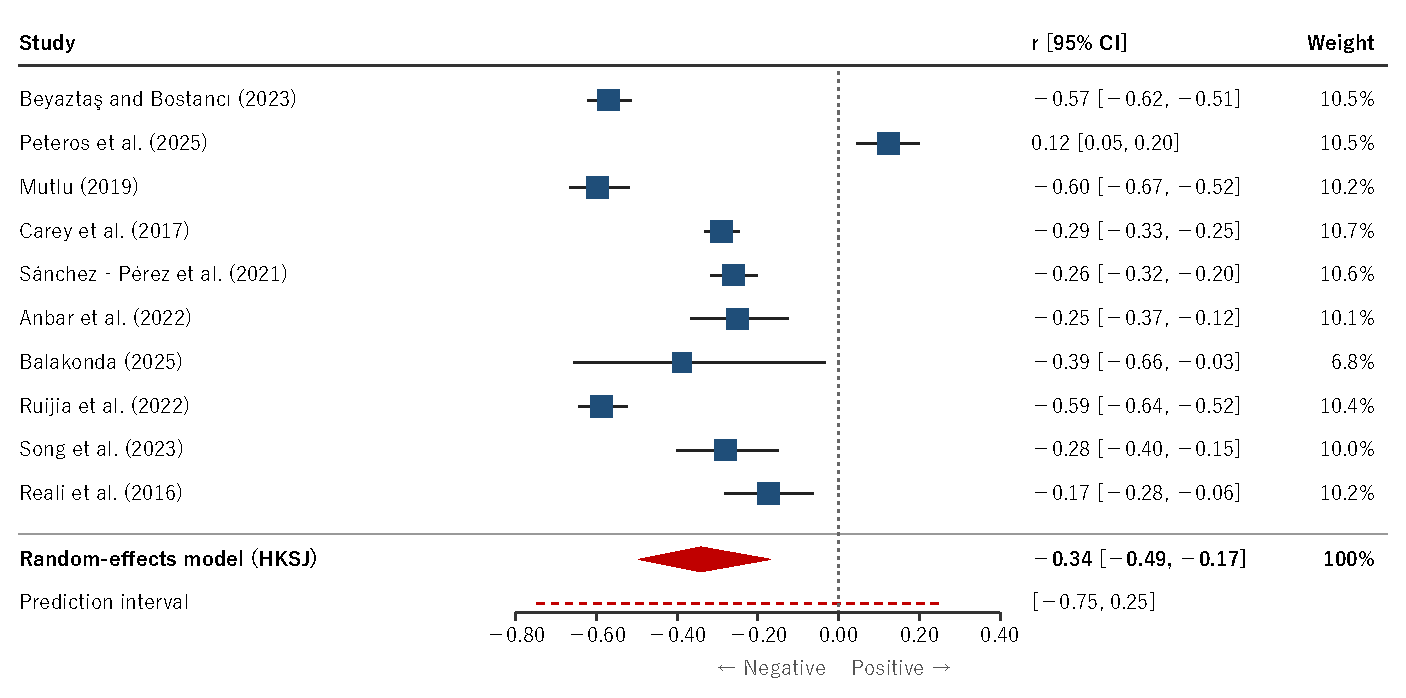
\includegraphics[width=\textwidth]{forest-en.pdf}\par\vspace{2pt}
{\tablefont\textbf{Figure 1.} Forest plot of individual and pooled effect sizes\par}{\tablefont Squares show study effect sizes (size proportional to weight), lines show 95\% confidence intervals, the diamond shows the pooled estimate, and the dashed line shows the prediction interval.\par}
\end{figure*}
The random-effects model yielded a pooled effect of \textit{r} = \ensuremath{-}.34, 95\% CI [\ensuremath{-}.49, \ensuremath{-}.17], \textit{t}(9) = \ensuremath{-}4.32, \textit{p} = .002, which corresponds to a moderate effect by conventional benchmarks. The fixed-effect estimate was \textit{r} = \ensuremath{-}.32. Table 3 summarizes these estimates.

\secn{3}{4}{Heterogeneity}
Heterogeneity was considerable, \textit{Q}(9) = 288.53, p < .001, \textit{I}² = 96.9\%, \textit{τ}² = 0.063. The 95\% prediction interval ranged from \ensuremath{-}.75 to .25.

\secn{3}{5}{Subgroup and Sensitivity Analyses}
For elementary (grades 1–6) samples, \textit{r} = \ensuremath{-}.44, 95\% CI [\ensuremath{-}.61, \ensuremath{-}.24] (\textit{k} = 6); for lower secondary (grades 7–9) samples, \textit{r} = \ensuremath{-}.11, 95\% CI [\ensuremath{-}1.00, 1.00] (\textit{k} = 2); for mixed grades samples, \textit{r} = \ensuremath{-}.24, 95\% CI [\ensuremath{-}.77, .48] (\textit{k} = 2). The difference between school levels was not statistically significant, \textit{Q}(2) = 4.84, \textit{p} = .089. Leave-one-out estimates ranged from \ensuremath{-}.39 to \ensuremath{-}.31. Egger’s test did not indicate funnel plot asymmetry (intercept = \ensuremath{-}1.96, \textit{p} = .680). The subgroup estimates are also shown in Table 3.

\begin{table*}[tb]
\centering
{\tablefont \textbf{Table 3.} Results of the Meta-Analysis\par}\vspace{2pt}
{\tablefont\renewcommand{\arraystretch}{1.12}
\begin{tabular}{lrrrrrrr}
\toprule
Model & \textit{k} & \textit{N} & \textit{r} & 95\% CI & \textit{p} & \textit{I}² (\%) & \textit{τ}² \\
\midrule
Random effects (HKSJ) & 10 & 5389 & \ensuremath{-}.34 & [\ensuremath{-}.49, \ensuremath{-}.17] & .002 & 96.9 & 0.063 \\
Fixed effect & 10 & 5389 & \ensuremath{-}.32 & [\ensuremath{-}.34, \ensuremath{-}.29] & < .001 & — & — \\
\hspace{1em}elementary (grades 1–6) & 6 & 2731 & \ensuremath{-}.44 & [\ensuremath{-}.61, \ensuremath{-}.24] & .003 & 95.4 & 0.049 \\
\hspace{1em}lower secondary (grades 7–9) & 2 & 642 & \ensuremath{-}.11 & [\ensuremath{-}1.00, 1.00] & .750 & 86.5 & 0.124 \\
\hspace{1em}mixed grades & 2 & 2016 & \ensuremath{-}.24 & [\ensuremath{-}.77, .48] & .151 & 73.5 & 0.006 \\
\bottomrule
\end{tabular}\par}
\vspace{2pt}{\tablefont\noindent \textit{Note.} \textit{k} = number of studies. HKSJ = Hartung–Knapp–Sidik–Jonkman confidence interval. 95\% prediction interval [\ensuremath{-}.75, .25].\par}
\end{table*}
\chap{4}{Discussion}
The random-effects model gave a pooled correlation of \textit{r} = \ensuremath{-}.34, 95\% CI [\ensuremath{-}.49, \ensuremath{-}.17], which is a moderate negative association by conventional benchmarks (Table 3). In the included studies, students who reported more mathematics anxiety tended to have lower mathematics achievement. Nine of the ten studies showed a negative correlation, and the exception was a study of eighth graders with a weak positive correlation [7]. The largest negative correlations came from studies of single grades in Turkey and China [1], [2], [4], while the largest sample showed a smaller correlation [5] (Fig. 1).

The results varied widely across studies (Fig. 1). Heterogeneity was very large (\textit{I}² = 96.9\%), and the 95\% prediction interval, [\ensuremath{-}.75, .25], was wide enough to include zero and weak positive values. This means that the pooled value should not be read as the expected correlation in every classroom. Differences in the anxiety scales, in the achievement measures (tests, report card grades or teacher-reported grades), and in the students sampled may all contribute (Table 2), but the present data do not allow us to say which of them explain the differences.

The subgroup analysis by school level suggested a stronger association in elementary samples (\textit{r} = \ensuremath{-}.44, \textit{k} = 6) than in middle school samples (\textit{r} = \ensuremath{-}.11, \textit{k} = 2) or in mixed-grade samples (\textit{r} = \ensuremath{-}.24, \textit{k} = 2). However, the difference between school levels was not statistically significant, \textit{Q}(2) = 4.84, \textit{p} = .089, the middle school estimate had a very wide interval, and the subgroups contained few studies. These results are exploratory, and we do not draw conclusions about why the association might differ by school level. Comparisons between passive and active control conditions did not apply to this correlational question. The sensitivity analysis, in which each study was removed in turn, gave pooled estimates between \ensuremath{-}.39 and \ensuremath{-}.31, so no single study determined the overall result. The Egger test did not indicate funnel plot asymmetry (intercept = \ensuremath{-}1.96, \textit{p} = .680), although a test with ten studies has little power.

For teachers of grades 1 to 9, the findings suggest paying attention to students' feelings about mathematics as well as to their scores. Students who look worried during mathematics lessons or tests may benefit from a calm classroom, clear explanations and chances to practise without pressure. At the same time, the data are correlational, so our results do not show that lowering anxiety will raise achievement, or that low achievement does not itself cause anxiety. Schools should therefore regard anxiety as one of several factors to watch, and should not rely on a single anxiety score to judge a student.

\chap{5}{Conclusion}
Across ten studies of students in primary and lower secondary schools, higher mathematics anxiety was associated with lower mathematics achievement, with a moderate pooled correlation of \textit{r} = \ensuremath{-}.34. The association varied greatly between studies and may be stronger in elementary samples, although this difference was not statistically significant. Because the evidence is correlational, small in number and automatically extracted, teachers can use it as a reason to attend to students' anxiety, but it does not show that reducing anxiety will by itself raise achievement.

This synthesis has several limitations. Only ten studies were included, and some had small samples [16] while others were large [5]. The studies came from different countries and used different anxiety scales and different achievement measures, which makes the combined estimate a rough summary. Some samples mixed students from several grades [5], [6], and one included students slightly older than the target range [6]. Subgroups contained as few as two studies, so subgroup estimates are imprecise. All of the included studies were correlational, so the direction of any relationship cannot be established.

The studies were found with a limited search of open-access sources, and the data were extracted automatically from the full texts. Every extracted number was checked against the text, but a human did not review the extraction, and several candidate studies could not be included because their full texts or correlations were not available or could not be read reliably. Where a study reported correlations for several outcomes, we used the one for the main achievement measure, and this choice could affect the result. For these reasons, the findings should be treated as provisional.

In addition, screening and data extraction were automated with a language model, and extracted numbers were verified only by matching them against the full text. A number can be present in the text yet belong to a different group or measure. Only open-access studies whose full texts could be retrieved were included; subscription-only and unpublished studies were not.

\chapx{Author notes}
This is a “Generative AI paper” produced automatically by the Society for Educational Data Analysis (SEDA) with generative AI. Large language models (claude-sonnet-5-5 (Claude Code, local)) were used to screen records, extract data, and draft the Introduction, Discussion, and Conclusion; all statistics were computed by software. The paper has not been peer reviewed.

Data and code are available at \url{https://github.com/k518-2026/MetaAnalysisToWP}. © 2026 Society for Educational Data Analysis (SEDA).

\chapx{References}
\noindent References marked with an asterisk indicate studies included in the meta-analysis.\par
{\fontsize{8.5pt}{10.5pt}\selectfont
\par\noindent\hangindent=2.4em\hangafter=1 \makebox[2.4em][l]{[1]}*D. İ. Beyaztaş and Y. Bostancı, “Investigating the Relationship Between Mathematics Anxiety and Mathematics Achievement of Primary School 4th Grade Students,” \textit{Kastamonu Eğitim Dergisi}, vol. 31, no. 3, pp. 498–512, 2023, doi: 10.24106/kefdergi.1336373.\par
\par\noindent\hangindent=2.4em\hangafter=1 \makebox[2.4em][l]{[2]}*Y. Mutlu, “Math Anxiety in Students With and Without Math Learning Difficulties,” \textit{lnternational Electronic Journal of Elementary Education}, vol. 11, no. 5, pp. 471–475, 2019, doi: 10.26822/iejee.2019553343.\par
\par\noindent\hangindent=2.4em\hangafter=1 \makebox[2.4em][l]{[3]}*N. Sánchez-Pérez, L. J. Fuentes, and C. González-Salinas, “Assessing math anxiety in elementary schoolchildren through a Spanish version of the Scale for Early Mathematics Anxiety (SEMA),” \textit{PLoS ONE}, vol. 16, no. 8, p. e0255777, 2021, doi: 10.1371/journal.pone.0255777.\par
\par\noindent\hangindent=2.4em\hangafter=1 \makebox[2.4em][l]{[4]}*Z. Ruijia, O. Talib, N. A. N. Burhanuddin, and W. Li, “The Effect of Math Self-Concept and Self-Efficacy on the Math Achievement of Sixth-Grade Primary School Students: The Mediating Role of Math Anxiety,” \textit{International Journal of Academic Research in Progressive Education and Development}, vol. 11, no. 3, 2022, doi: 10.6007/ijarped/v11-i3/14721.\par
\par\noindent\hangindent=2.4em\hangafter=1 \makebox[2.4em][l]{[5]}*E. Carey, A. Devine, F. Hill, and D. Szűcs, “Differentiating anxiety forms and their role in academic performance from primary to secondary school,” \textit{PLoS ONE}, vol. 12, no. 3, p. e0174418, 2017, doi: 10.1371/journal.pone.0174418.\par
\par\noindent\hangindent=2.4em\hangafter=1 \makebox[2.4em][l]{[6]}*F. Reali, W. Jiménez-Leal, C. Maldonado-Carreño, A. Devine, and D. Szűcs, “Examining the link between math anxiety and math performance in Colombian students,” \textit{Revista Colombiana de Psicología}, vol. 25, no. 2, 2016, doi: 10.15446/rcp.v25n2.54532.\par
\par\noindent\hangindent=2.4em\hangafter=1 \makebox[2.4em][l]{[7]}*E. D. L. Peteros, L. B. Tandoc, M. H. Palapar, R. C. Adlaw, and C. M. Fuentes, “Mathematics anxiety as a moderator between self-esteem and mathematics achievement among Filipino Grade 8 students,” \textit{STEM Education}, vol. 5, no. 5, pp. 933–953, 2025, doi: 10.3934/steme.2025041.\par
\par\noindent\hangindent=2.4em\hangafter=1 \makebox[2.4em][l]{[8]}R. DerSimonian and N. Laird, “Meta-analysis in clinical trials,” \textit{Controlled Clinical Trials}, vol. 7, no. 3, pp. 177–188, 1986, doi: 10.1016/0197-2456(86)90046-2.\par
\par\noindent\hangindent=2.4em\hangafter=1 \makebox[2.4em][l]{[9]}J. Hartung and G. Knapp, “A refined method for the meta-analysis of controlled clinical trials with binary outcome,” \textit{Statistics in Medicine}, vol. 20, no. 24, pp. 3875–3889, 2001, doi: 10.1002/sim.1009.\par
\par\noindent\hangindent=2.4em\hangafter=1 \makebox[2.4em][l]{[10]}J. IntHout, J. P. A. Ioannidis, and G. F. Borm, “The Hartung-Knapp-Sidik-Jonkman method for random effects meta-analysis is straightforward and considerably outperforms the standard DerSimonian-Laird method,” \textit{BMC Medical Research Methodology}, vol. 14, Art. no. 25, 2014, doi: 10.1186/1471-2288-14-25.\par
\par\noindent\hangindent=2.4em\hangafter=1 \makebox[2.4em][l]{[11]}J. P. T. Higgins and S. G. Thompson, “Quantifying heterogeneity in a meta-analysis,” \textit{Statistics in Medicine}, vol. 21, no. 11, pp. 1539–1558, 2002, doi: 10.1002/sim.1186.\par
\par\noindent\hangindent=2.4em\hangafter=1 \makebox[2.4em][l]{[12]}M. Egger, G. Davey Smith, M. Schneider, and C. Minder, “Bias in meta-analysis detected by a simple, graphical test,” \textit{BMJ}, vol. 315, no. 7109, pp. 629–634, 1997, doi: 10.1136/bmj.315.7109.629.\par
\par\noindent\hangindent=2.4em\hangafter=1 \makebox[2.4em][l]{[13]}J. Cohen, \textit{Statistical Power Analysis for the Behavioral Sciences}, 2nd ed. Lawrence Erlbaum Associates, 1988.\par
\par\noindent\hangindent=2.4em\hangafter=1 \makebox[2.4em][l]{[14]}M. Borenstein, L. V. Hedges, J. P. T. Higgins, and H. R. Rothstein, \textit{Introduction to Meta-Analysis}, Wiley, 2009, doi: 10.1002/9780470743386.\par
\par\noindent\hangindent=2.4em\hangafter=1 \makebox[2.4em][l]{[15]}*N. Anbar, L. Cheie, and L. Visu-Petra, “Math Anxiety, Math Achievement and Gender Differences among Primary School Children and their Parents from Palestine,” \textit{International Journal of Learning Teaching and Educational Research}, vol. 21, no. 8, pp. 326–334, 2022, doi: 10.26803/ijlter.21.8.19.\par
\par\noindent\hangindent=2.4em\hangafter=1 \makebox[2.4em][l]{[16]}*V. Balakonda, “Exploring the Relationship between Mathematics Anxiety, Interest, and Academic Achievement among Secondary School Students,” \textit{Journal of Informatics Education and Research}, 2025. [Online]. Available: \url{https://jier.org/index.php/journal/article/view/2800}\par
\par\noindent\hangindent=2.4em\hangafter=1 \makebox[2.4em][l]{[17]}*S. Song, T. Li, M. Quintero, and Z. Wang, “The link between math anxiety and math achievement: The role of afterschool learning,” \textit{Journal of Numerical Cognition}, vol. 9, no. 3, pp. 418–432, 2023, doi: 10.5964/jnc.11325.\par
}
\end{document}
